\section{Introduction}

\label{sec:intro}

\begin{frame}{Indirect methods for VBL}
	
	Visual Based Localization (\textbf{VBL}) aims to recover the pose or position of a visual input query according to a known reference~\cite{Piasco2017}.
	\vfill	
	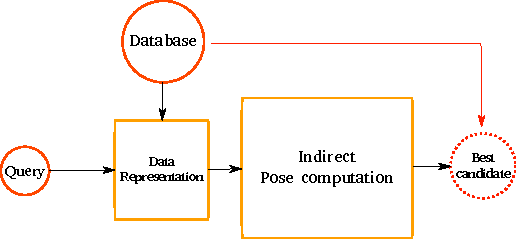
\includegraphics{vect/keys_comp_indirect.pdf}
	
\end{frame}

\begin{frame}{CNN for data representation}
	
	\vfill	
	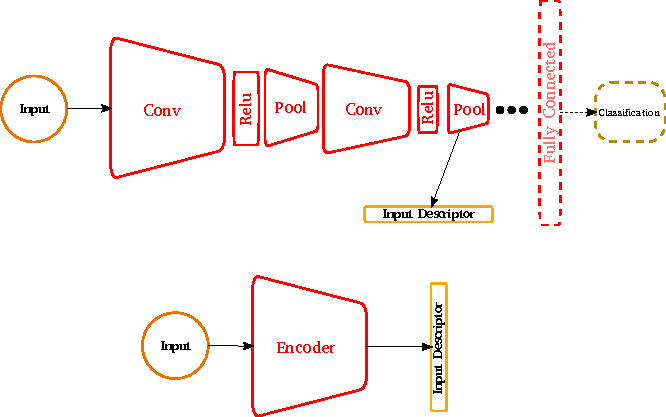
\includegraphics{vect/encodeur.pdf}
	\vfill	
		
\end{frame}


\begin{frame}{Proposed framework}
	\vfill
	\begin{block}{Framework}
		\centering
		\begin{tabular}{c | c}
			\textbf{Training data type} & \textbf{Testing data type} \\
			\hline
			\textbf<2>{RGB + Depth} & \textbf<3>{RGB}  \\
		\end{tabular}
	\end{block}
	\vfill
	\begin{figure}[t]
		\centering
		\uncover<2->{
		\begin{minipage}[b]{0.65\linewidth}
			\centering
			{\footnotesize \textbf{Multi-modal} training dataset}	
	
			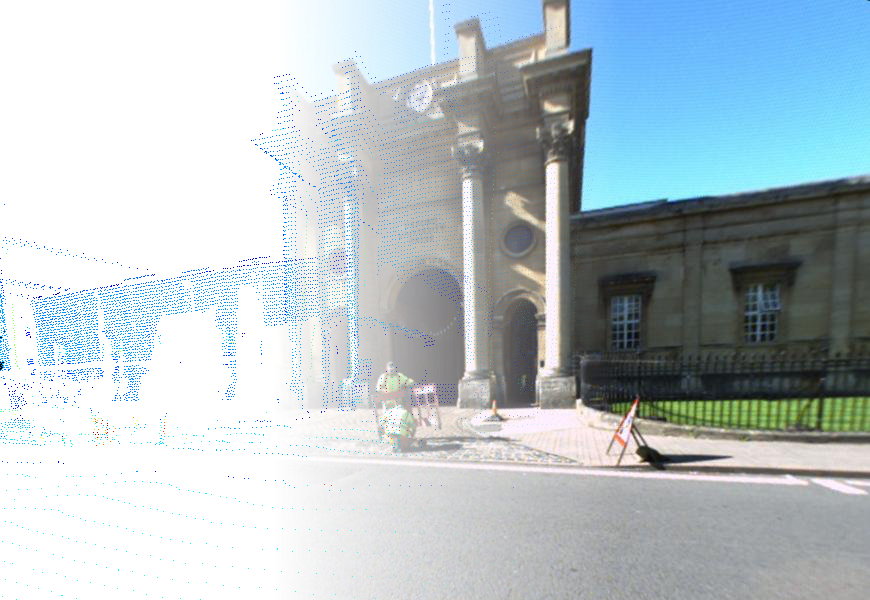
\includegraphics[width=0.51\linewidth]{images/intro_fig/mod0.png}
			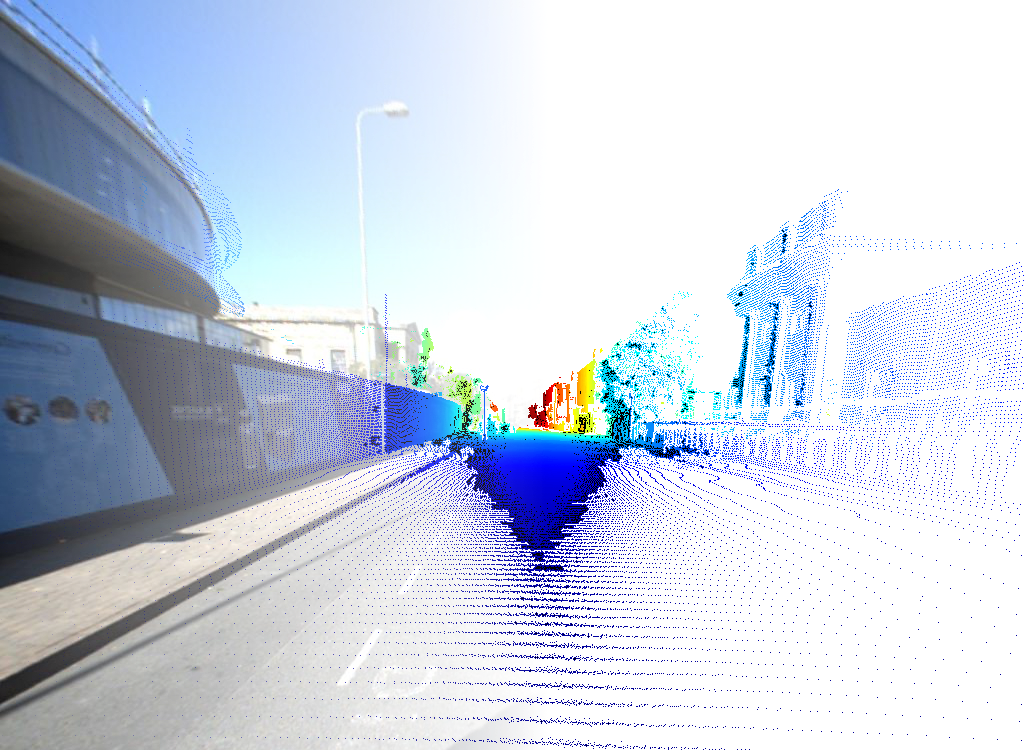
\includegraphics[width=0.47\linewidth]{images/intro_fig/mod1.png}
		\end{minipage}
		}
		\uncover<3>{
		\begin{minipage}[b]{0.32\linewidth}
			\centering
			{\footnotesize \textbf{Single modality} data at test time}
	
			
\includegraphics[width=0.85\linewidth]{images/intro_fig/q.jpg}
		\end{minipage}
		}
	\end{figure}
\end{frame}
